\documentclass{article}\usepackage[]{graphicx}\usepackage[]{color}
%% maxwidth is the original width if it is less than linewidth
%% otherwise use linewidth (to make sure the graphics do not exceed the margin)
\makeatletter
\def\maxwidth{ %
  \ifdim\Gin@nat@width>\linewidth
    \linewidth
  \else
    \Gin@nat@width
  \fi
}
\makeatother

\definecolor{fgcolor}{rgb}{0.345, 0.345, 0.345}
\newcommand{\hlnum}[1]{\textcolor[rgb]{0.686,0.059,0.569}{#1}}%
\newcommand{\hlstr}[1]{\textcolor[rgb]{0.192,0.494,0.8}{#1}}%
\newcommand{\hlcom}[1]{\textcolor[rgb]{0.678,0.584,0.686}{\textit{#1}}}%
\newcommand{\hlopt}[1]{\textcolor[rgb]{0,0,0}{#1}}%
\newcommand{\hlstd}[1]{\textcolor[rgb]{0.345,0.345,0.345}{#1}}%
\newcommand{\hlkwa}[1]{\textcolor[rgb]{0.161,0.373,0.58}{\textbf{#1}}}%
\newcommand{\hlkwb}[1]{\textcolor[rgb]{0.69,0.353,0.396}{#1}}%
\newcommand{\hlkwc}[1]{\textcolor[rgb]{0.333,0.667,0.333}{#1}}%
\newcommand{\hlkwd}[1]{\textcolor[rgb]{0.737,0.353,0.396}{\textbf{#1}}}%
\let\hlipl\hlkwb

\usepackage{framed}
\makeatletter
\newenvironment{kframe}{%
 \def\at@end@of@kframe{}%
 \ifinner\ifhmode%
  \def\at@end@of@kframe{\end{minipage}}%
  \begin{minipage}{\columnwidth}%
 \fi\fi%
 \def\FrameCommand##1{\hskip\@totalleftmargin \hskip-\fboxsep
 \colorbox{shadecolor}{##1}\hskip-\fboxsep
     % There is no \\@totalrightmargin, so:
     \hskip-\linewidth \hskip-\@totalleftmargin \hskip\columnwidth}%
 \MakeFramed {\advance\hsize-\width
   \@totalleftmargin\z@ \linewidth\hsize
   \@setminipage}}%
 {\par\unskip\endMakeFramed%
 \at@end@of@kframe}
\makeatother

\definecolor{shadecolor}{rgb}{.97, .97, .97}
\definecolor{messagecolor}{rgb}{0, 0, 0}
\definecolor{warningcolor}{rgb}{1, 0, 1}
\definecolor{errorcolor}{rgb}{1, 0, 0}
\newenvironment{knitrout}{}{} % an empty environment to be redefined in TeX

\usepackage{alltt}
\usepackage[backend=bibtex, sorting=none]{biblatex}
\usepackage{hyperref}
\bibliography{references}
\begin{filecontents*}{references.bib}
@article{Tzelepis:2016ix,
author = {Tzelepis, Konstantinos and Koike-Yusa, Hiroko and De Braekeleer, Etienne and Li, Yilong and Metzakopian, Emmanouil and Dovey, Oliver M and Mupo, Annalisa and Grinkevich, Vera and Li, Meng and Mazan, Milena and Gozdecka, Malgorzata and Ohnishi, Shuhei and Cooper, Jonathan and Patel, Miten and McKerrell, Thomas and Chen, Bin and Domingues, Ana Filipa and Gallipoli, Paolo and Teichmann, Sarah and Ponstingl, Hannes and McDermott, Ultan and Saez-Rodriguez, Julio and Huntly, Brian J P and Iorio, Francesco and Pina, Cristina and Vassiliou, George S and Yusa, Kosuke},
title = {{A CRISPR Dropout Screen Identifies Genetic Vulnerabilities and Therapeutic Targets in Acute Myeloid Leukemia.}},
journal = {Cell reports},
year = {2016},
volume = {17},
number = {4},
pages = {1193--1205},
month = oct
}

@article{Iorio:2017,
author = {Iorio, Francesco and Behan, Fiona M and Goncalves, Emanuel and Beaver, Charlotte and Ansari, Rizwan  and Pooley, Rachel and Wilkinson, Piers and Harper, Sarah and Stronach, Euan and Saez-Rodriguez, Julio and Yusa, Kosuke and Garnett, Mathew J
},
title = {{Unsupervised correction of gene-independent cell responses to CRISPR-Cas9 targeting}},
journal = {revision},
volume = {0},
number = {0},
pages = {0--0},
month = Dec
}

@article{Li:2014kt,
author = {Li, Wei and Xu, Han and Xiao, Tengfei and Cong, Le and Love, Michael I and Zhang, Feng and Irizarry, Rafael A and Liu, Jun S and Brown, Myles and Liu, X Shirley},
title = {{MAGeCK enables robust identification of essential genes from genome-scale CRISPR/Cas9 knockout screens.}},
journal = {Genome Biology},
year = {2014},
volume = {15},
number = {12},
pages = {554}
}

@article{Hart:2016ja,
author = {Hart, Traver and Moffat, Jason},
title = {{BAGEL: a computational framework for identifying essential genes from pooled library screens.}},
journal = {BMC bioinformatics},
year = {2016},
volume = {17},
pages = {164},
month = apr
}

@article{Subramanian:2005wu,
author = {Subramanian, A and Tamayo, P and Mootha, VK and Mukherjee, S and Ebert, BL and Gillette, MA and Paulovich, A and Pomeroy, SL and Golub, TR and Lander, ES},
title = {{Gene set enrichment analysis: a knowledge-based approach for interpreting genome-wide expression profiles}},
journal = {Proceedings of the National Academy of Sciences of the United States of America},
year = {2005},
volume = {102},
number = {43},
pages = {15545}
}

@article{Iorio:2016ds,
author = {Iorio, Francesco and Knijnenburg, Theo A and Vis, Daniel J and Bignell, Graham R and Menden, Michael P and Schubert, Michael and Aben, Nanne and Gon{\c c}alves, Emanuel and Barthorpe, Syd and Lightfoot, Howard and Cokelaer, Thomas and Greninger, Patricia and van Dyk, Ewald and Chang, Han and de Silva, Heshani and Heyn, Holger and Deng, Xianming and Egan, Regina K and Liu, Qingsong and Mironenko, Tatiana and Mitropoulos, Xeni and Richardson, Laura and Wang, Jinhua and Zhang, Tinghu and Moran, Sebastian and Sayols, Sergi and Soleimani, Maryam and Tamborero, David and Lopez-Bigas, Nuria and Ross-Macdonald, Petra and Esteller, Manel and Gray, Nathanael S and Haber, Daniel A and Stratton, Michael R and Benes, Cyril H and Wessels, Lodewyk F A and Saez-Rodriguez, Julio and McDermott, Ultan and Garnett, Mathew J},
title = {{A Landscape of Pharmacogenomic Interactions in Cancer.}},
journal = {Cell},
year = {2016},
month = jul
}

\end{filecontents*}
\IfFileExists{upquote.sty}{\usepackage{upquote}}{}
\begin{document}
\title{CRISPRcleanR: An R package for unsupervised identification and correction of gene independent cell responses to CRISPR-cas9 targeting}
\author{Francesco Iorio, fi1@sanger.ac.uk}
\maketitle
\section{Quick start}

\subsection{Installation}
 
First, you need to install and load the devtools package. You can do this from CRAN. Invoke R and then type:
 
\begin{knitrout}
\definecolor{shadecolor}{rgb}{0.969, 0.969, 0.969}\color{fgcolor}\begin{kframe}
\begin{alltt}
\hlkwd{install.packages}\hlstd{(}\hlstr{"devtools"}\hlstd{)}
\hlkwd{library}\hlstd{(devtools)}
\end{alltt}
\end{kframe}
\end{knitrout}

Secondly, install CRISPRcleanR with the following command:

\begin{knitrout}
\definecolor{shadecolor}{rgb}{0.969, 0.969, 0.969}\color{fgcolor}\begin{kframe}
\begin{alltt}
\hlkwd{install_github}\hlstd{(}\hlstr{"francescojm/CRISPRcleanR"}\hlstd{)}
\end{alltt}
\end{kframe}
\end{knitrout}

\subsection{Raw sgRNA count median-ratio normalisation and computation of sgRNAs' log fold-changes}
 
Load CRISPRcleanR.

 
\begin{knitrout}
\definecolor{shadecolor}{rgb}{0.969, 0.969, 0.969}\color{fgcolor}\begin{kframe}
\begin{alltt}
    \hlkwd{library}\hlstd{(CRISPRcleanR)}
\end{alltt}


{\ttfamily\noindent\itshape\color{messagecolor}{\#\# Loading required package: stringr}}

{\ttfamily\noindent\itshape\color{messagecolor}{\#\# Loading required package: DNAcopy}}

{\ttfamily\noindent\itshape\color{messagecolor}{\#\# Loading required package: pROC}}

{\ttfamily\noindent\itshape\color{messagecolor}{\#\# Type 'citation("{}pROC"{})' for a citation.}}

{\ttfamily\noindent\itshape\color{messagecolor}{\#\# \\\#\# Attaching package: 'pROC'}}

{\ttfamily\noindent\itshape\color{messagecolor}{\#\# The following objects are masked from 'package:stats':\\\#\# \\\#\#\ \ \ \  cov, smooth, var}}

{\ttfamily\noindent\itshape\color{messagecolor}{\#\# Loading required package: pracma}}\end{kframe}
\end{knitrout}


% 
\textbf{Step 1:} Load your sgRNA library annotation. In this example we will use a built in data frame containing the annotation of the SANGER v1.0 library, introduced in \cite{Tzelepis:2016ix}:
\begin{knitrout}
\definecolor{shadecolor}{rgb}{0.969, 0.969, 0.969}\color{fgcolor}\begin{kframe}
\begin{alltt}
\hlkwd{data}\hlstd{(KY_Library_v1.0)}
\end{alltt}
\end{kframe}
\end{knitrout}
% 
To use your own library annotation you will have to store it into a data frame with the same format of the \texttt{KY\char`_Library\char`_v1.0} (detailed in the corresponding entry of the reference manual of the CRISPRcleanR package).\\

\textbf{Step 2:} Store the path of the tsv file containing your sgRNAs' raw counts in a temporary variable. In this example we will use counts generated upon a CRISPR-Cas9 pooled drop-out screen (described in \cite{Iorio:2017}) built in this package, for an example immortalised human cancer cell line (HT-29)

\begin{knitrout}
\definecolor{shadecolor}{rgb}{0.969, 0.969, 0.969}\color{fgcolor}\begin{kframe}
\begin{alltt}
 \hlstd{fn}\hlkwb{<-}\hlkwd{paste}\hlstd{(}\hlkwd{system.file}\hlstd{(}\hlstr{'extdata'}\hlstd{,}\hlkwc{package} \hlstd{=} \hlstr{'CRISPRcleanR'}\hlstd{),}
           \hlstr{'/HT-29_counts.tsv'}\hlstd{,}\hlkwc{sep}\hlstd{=}\hlstr{''}\hlstd{)}
\end{alltt}
\end{kframe}
\end{knitrout}

The tsv file with the sgRNAs' raw counts must be formatted as specified in the reference manual entry of the \texttt{ccr.NormfoldChanges} function.\\
 
\textbf{Step 3:} Perform a median-ratio normalisation of raw counts and compute sgRNAs' log fold-changes (in this example we will exclude sgRNAs with less than 30 reads in the plasmid sample).

\begin{knitrout}
\definecolor{shadecolor}{rgb}{0.969, 0.969, 0.969}\color{fgcolor}\begin{kframe}
\begin{alltt}
\hlstd{normANDfcs}\hlkwb{<-}\hlkwd{ccr.NormfoldChanges}\hlstd{(fn,}
                                 \hlkwc{min_reads}\hlstd{=}\hlnum{30}\hlstd{,}
                                 \hlkwc{EXPname}\hlstd{=}\hlstr{'HT-29'}\hlstd{,}
                                 \hlkwc{libraryAnnotation}\hlstd{=KY_Library_v1.0)}
\end{alltt}
\end{kframe}
\includegraphics[width=\maxwidth]{figure/Norm_and_fc-1} 

\includegraphics[width=\maxwidth]{figure/Norm_and_fc-2} 

\end{knitrout}

This function returns a list of two data frames containing, normalised counts and log fold-changes, respectively, and it saves them as Robjects in a user defined directory (specified by the parameter \texttt{outdir}, which is set to \texttt{'./'} by default).

\begin{knitrout}\small
\definecolor{shadecolor}{rgb}{0.969, 0.969, 0.969}\color{fgcolor}\begin{kframe}
\begin{alltt}
\hlkwd{head}\hlstd{(normANDfcs}\hlopt{$}\hlstd{norm_counts)}
\end{alltt}
\begin{verbatim}
##                                             sgRNA gene ERS717283.plasmid
## 1 A1BG_CCDS12976.1_ex3_19:58862927-58862950:-_5-1 A1BG         292.14621
## 2 A1BG_CCDS12976.1_ex4_19:58863655-58863678:+_5-2 A1BG         151.02032
## 3 A1BG_CCDS12976.1_ex4_19:58863697-58863720:-_5-3 A1BG         209.08503
## 4 A1BG_CCDS12976.1_ex4_19:58863866-58863889:+_5-4 A1BG         110.40106
## 5 A1BG_CCDS12976.1_ex5_19:58864367-58864390:-_5-5 A1BG          95.81979
## 6  A1CF_CCDS7241.1_ex6_10:52588014-52588037:-_5-1 A1CF          60.92889
##   HT29_c904R1 HT29_c904R2 HT29_c904R3
## 1   308.05192   354.89835   305.56806
## 2   145.38048   113.16912   166.47364
## 3   280.97793   203.70441   223.03071
## 4    80.31191    64.05372    78.74023
## 5    78.71932   123.80701   103.32157
## 6    47.77762    76.50232    59.75464
\end{verbatim}
\begin{alltt}
\hlkwd{head}\hlstd{(normANDfcs}\hlopt{$}\hlstd{logFCs)}
\end{alltt}
\begin{verbatim}
##                                             sgRNA gene HT29_c904R1
## 1 A1BG_CCDS12976.1_ex3_19:58862927-58862950:-_5-1 A1BG  0.07635566
## 2 A1BG_CCDS12976.1_ex4_19:58863655-58863678:+_5-2 A1BG -0.05472442
## 3 A1BG_CCDS12976.1_ex4_19:58863697-58863720:-_5-3 A1BG  0.42548611
## 4 A1BG_CCDS12976.1_ex4_19:58863866-58863889:+_5-4 A1BG -0.45663336
## 5 A1BG_CCDS12976.1_ex5_19:58864367-58864390:-_5-5 A1BG -0.28197989
## 6  A1CF_CCDS7241.1_ex6_10:52588014-52588037:-_5-1 A1CF -0.34756262
##   HT29_c904R2 HT29_c904R3
## 1  0.28027938  0.06469488
## 2 -0.41467098  0.14010902
## 3 -0.03752168  0.09293733
## 4 -0.78070106 -0.48496821
## 5  0.36800353  0.10820208
## 6  0.32598467 -0.02784489
\end{verbatim}
\end{kframe}
\end{knitrout}
 
\textbf{IMPORTANT:} if there are control replicates in your sgRNAs count file their number must be specified by in the parameter \texttt{ncontrols} (equal to 1 by default) of the \texttt{ccr.NormfoldChanges} function.
 
\subsection{Genome sorting of sgRNAs' log fold-changes and their correction for gene independent responses to CRISPR-Cas9 targeting}

\textbf{Step 1:} Map genome-wide sgRNAs' log fold changes (averaged across replicates) on the genome, sorted according to the of their targeted gene on the chromosomes.
 
\begin{knitrout}
\definecolor{shadecolor}{rgb}{0.969, 0.969, 0.969}\color{fgcolor}\begin{kframe}
\begin{alltt}
\hlstd{gwSortedFCs}\hlkwb{<-}
     \hlkwd{ccr.logFCs2chromPos}\hlstd{(normANDfcs}\hlopt{$}\hlstd{logFCs,KY_Library_v1.0)}
\end{alltt}
\end{kframe}
\end{knitrout}
 
\begin{knitrout}\small
\definecolor{shadecolor}{rgb}{0.969, 0.969, 0.969}\color{fgcolor}\begin{kframe}
\begin{alltt}
\hlkwd{head}\hlstd{(gwSortedFCs)}
\end{alltt}
\begin{verbatim}
##                                          CHR startp   endp  genes
## SAMD11_CCDS2.2_ex3_1:871254-871277:+_5-1   1 871254 871277 SAMD11
## SAMD11_CCDS2.2_ex4_1:874451-874474:-_5-2   1 874451 874474 SAMD11
## SAMD11_CCDS2.2_ex4_1:874487-874510:+_5-3   1 874487 874510 SAMD11
## SAMD11_CCDS2.2_ex5_1:874693-874716:+_5-4   1 874693 874716 SAMD11
## SAMD11_CCDS2.2_ex6_1:876601-876624:-_5-5   1 876601 876624 SAMD11
## NOC2L_CCDS3.1_ex8_1:887388-887411:+_5-1    1 887388 887411  NOC2L
##                                                avgFC       BP
## SAMD11_CCDS2.2_ex3_1:871254-871277:+_5-1 -0.12965287 871265.5
## SAMD11_CCDS2.2_ex4_1:874451-874474:-_5-2  0.09329615 874462.5
## SAMD11_CCDS2.2_ex4_1:874487-874510:+_5-3  0.25286616 874498.5
## SAMD11_CCDS2.2_ex5_1:874693-874716:+_5-4 -0.05128489 874704.5
## SAMD11_CCDS2.2_ex6_1:876601-876624:-_5-5 -0.02110076 876612.5
## NOC2L_CCDS3.1_ex8_1:887388-887411:+_5-1  -1.27571756 887399.5
\end{verbatim}
\end{kframe}
\end{knitrout}
% 
\textbf{Step 2:} Identify and correct biased sgRNAs' log fold-changes putatively due to gene independent responses to CRISPR-Cas9 targeting, using the \texttt{ccr.GWclean} function. This function calls iteratively the \texttt{ccr.cleanChrm} function, which performs the correction on an individual chromosome). In this example we are using a completely unsuerpvised approach and correcting chromosomal segments of equal sgRNA log fold-changes if they include sgRNAs targeting at least 3 different genes, and without making any assumption on gene essentiality, nor knowing \textit{a priori} the copy number status of the included genes \cite{Iorio:2017}.

\begin{knitrout}
\definecolor{shadecolor}{rgb}{0.969, 0.969, 0.969}\color{fgcolor}\begin{kframe}
\begin{alltt}
\hlstd{correctedFCs}\hlkwb{<-}\hlkwd{ccr.GWclean}\hlstd{(gwSortedFCs,}\hlkwc{display}\hlstd{=}\hlnum{TRUE}\hlstd{,}\hlkwc{label}\hlstd{=}\hlstr{'HT-29'}\hlstd{)}
\end{alltt}
\end{kframe}
\end{knitrout}

The corrected sgRNAs fold-changes are returned in a list (as a data frame), together with the annotation of the identified segments (in another data frame) and a vector of strings containing all the gemome-sorted sgRNAs' identifiers.
 
\begin{knitrout}\small
\definecolor{shadecolor}{rgb}{0.969, 0.969, 0.969}\color{fgcolor}\begin{kframe}
\begin{alltt}
     \hlkwd{head}\hlstd{(correctedFCs}\hlopt{$}\hlstd{corrected_logFCs)}
\end{alltt}
\begin{verbatim}
##                                          CHR startp   endp  genes
## SAMD11_CCDS2.2_ex3_1:871254-871277:+_5-1   1 871254 871277 SAMD11
## SAMD11_CCDS2.2_ex4_1:874451-874474:-_5-2   1 874451 874474 SAMD11
## SAMD11_CCDS2.2_ex4_1:874487-874510:+_5-3   1 874487 874510 SAMD11
## SAMD11_CCDS2.2_ex5_1:874693-874716:+_5-4   1 874693 874716 SAMD11
## SAMD11_CCDS2.2_ex6_1:876601-876624:-_5-5   1 876601 876624 SAMD11
## NOC2L_CCDS3.1_ex8_1:887388-887411:+_5-1    1 887388 887411  NOC2L
##                                                avgFC       BP correction
## SAMD11_CCDS2.2_ex3_1:871254-871277:+_5-1 -0.12965287 871265.5          0
## SAMD11_CCDS2.2_ex4_1:874451-874474:-_5-2  0.09329615 874462.5          0
## SAMD11_CCDS2.2_ex4_1:874487-874510:+_5-3  0.25286616 874498.5          0
## SAMD11_CCDS2.2_ex5_1:874693-874716:+_5-4 -0.05128489 874704.5          0
## SAMD11_CCDS2.2_ex6_1:876601-876624:-_5-5 -0.02110076 876612.5          0
## NOC2L_CCDS3.1_ex8_1:887388-887411:+_5-1  -1.27571756 887399.5          0
##                                          correctedFC
## SAMD11_CCDS2.2_ex3_1:871254-871277:+_5-1 -0.12965287
## SAMD11_CCDS2.2_ex4_1:874451-874474:-_5-2  0.09329615
## SAMD11_CCDS2.2_ex4_1:874487-874510:+_5-3  0.25286616
## SAMD11_CCDS2.2_ex5_1:874693-874716:+_5-4 -0.05128489
## SAMD11_CCDS2.2_ex6_1:876601-876624:-_5-5 -0.02110076
## NOC2L_CCDS3.1_ex8_1:887388-887411:+_5-1  -1.27571756
\end{verbatim}
\end{kframe}
\end{knitrout}
% 
Details on how the data frame with the corrected sgRNAs' log fold-changes should be interpreted can be found in the entry of the \texttt{ccr.GWclean} function, of the package reference manual.\\
 
This function also produces one plot per chromosome, with segments of sgRNAs' equal log fold-change before and after the correction. An example of these plot is reported below: chromosome 8, in HT-29, showing a region containing \textit{MYC}, which is highly biased toward consistent negative fold-changes.
 
\begin{knitrout}
\definecolor{shadecolor}{rgb}{0.969, 0.969, 0.969}\color{fgcolor}
\includegraphics[width=\maxwidth]{figure/correction_chrm8-1} 

\end{knitrout}
 
\subsection{Correcting sgRNAs' treatment counts for mean-variance modeling}
In order to apply the inverse transformation described in \cite{Iorio:2017}, deriving corrected normalised sgRNAs' treatment counts from CRISPRcleanR corrected log fold-changes, it is sufficient to run the function \texttt{ccr.correctCounts} as follows:

\begin{knitrout}
\definecolor{shadecolor}{rgb}{0.969, 0.969, 0.969}\color{fgcolor}\begin{kframe}
\begin{alltt}
\hlstd{correctedCounts}\hlkwb{<-}\hlkwd{ccr.correctCounts}\hlstd{(}\hlstr{'HT-29'}\hlstd{,}
                                    \hlstd{normANDfcs}\hlopt{$}\hlstd{norm_counts,}
                                    \hlstd{correctedFCs,}
                                    \hlstd{KY_Library_v1.0,}
                                    \hlkwc{minTargetedGenes}\hlstd{=}\hlnum{3}\hlstd{,}
                                    \hlkwc{OutDir}\hlstd{=}\hlstr{'./'}\hlstd{)}
\end{alltt}
\end{kframe}
\end{knitrout}
% 
Together with the plasmid counts, the corrected treatment counts can be used to compute depletion singificance scores with a mean-variance modeling approach (such that implemented in MAGeCK\cite{Li:2014kt}). 

\begin{knitrout}
\definecolor{shadecolor}{rgb}{0.969, 0.969, 0.969}\color{fgcolor}\begin{kframe}
\begin{alltt}
\hlkwd{head}\hlstd{(correctedCounts)}
\end{alltt}
\begin{verbatim}
##                                             sgRNA gene ERS717283.plasmid
## 1 A1BG_CCDS12976.1_ex3_19:58862927-58862950:-_5-1 A1BG         292.14621
## 2 A1BG_CCDS12976.1_ex4_19:58863655-58863678:+_5-2 A1BG         151.02032
## 3 A1BG_CCDS12976.1_ex4_19:58863697-58863720:-_5-3 A1BG         209.08503
## 4 A1BG_CCDS12976.1_ex4_19:58863866-58863889:+_5-4 A1BG         110.40106
## 5 A1BG_CCDS12976.1_ex5_19:58864367-58864390:-_5-5 A1BG          95.81979
## 6  A1CF_CCDS7241.1_ex6_10:52588014-52588037:-_5-1 A1CF          60.92889
##   HT29_c904R1 HT29_c904R2 HT29_c904R3
## 1   309.77863   356.73522   307.28892
## 2   144.74469   112.89328   165.60212
## 3   280.34458   203.51866   222.73301
## 4    80.64680    64.52159    79.08797
## 5    78.22697   122.47062   102.36866
## 6    45.21299    71.83850    56.31473
\end{verbatim}
\end{kframe}
\end{knitrout}
 
This function also saves the correctedCounts as Rdata object at the location specified by the parameter \texttt{OutDir}.
To run MAGeCK, using these corrected sgRNAs' counts you will need to save them as a tsv file, which will be ued as input for MAGeCK:

\begin{knitrout}
\definecolor{shadecolor}{rgb}{0.969, 0.969, 0.969}\color{fgcolor}\begin{kframe}
\begin{alltt}
\hlkwd{write.table}\hlstd{(correctedCounts,}
             \hlkwc{quote}\hlstd{=}\hlnum{FALSE}\hlstd{,}
             \hlkwc{row.names} \hlstd{=} \hlnum{FALSE}\hlstd{,}
             \hlkwc{sep}\hlstd{=}\hlstr{'\textbackslash{}t'}\hlstd{,}
             \hlkwc{file}\hlstd{=}\hlstr{'./HT-29_mgk_input_corrected.tsv'}\hlstd{)}
\end{alltt}
\end{kframe}
\end{knitrout}

 
\textbf{IMPORTANT:} the corrected sgRNAs' counts are already median-normalised,
therefore, when executing MAGeCK, the parameter \texttt{--norm-method} should be set to \texttt{none}.
 
\section{Visualisation and assessment of Results}
 
\subsection{Classification performances of reference sets of genes (or sgRNAs) based on depletion log fold-changes}

To perform a basic quality control assessment of your data it is possible to test the genome-wide profile of sgRNAs' depletion log fold-changes (logFCs) (or gene depletion logFCs, averaged across targeting sgRNAs) as a classifier of reference sets of core-fitness essential (CFE) and non-essential genes.\\

What you need for this is a named vector of sgRNAs (or gene) logFCs and two reference gene sets (respectively for positive and negative cases). In this example we make use of a precomputed essentiality profile from the builtin data object \texttt{EPLC.272HcorrectedFCs}. This is a list containing corrected sgRNAs log fold-changes and segment annotations for an example cell line (EPLC-272H), obtained using the \texttt{ccr.GWclean} function, as detailed in its reference manual entry. However the data frame containing the corrected log fold-changes, included in this list, reports also the original sgRNAs logFC (column \texttt{avgFC}), which will be used in this example.
 
\begin{knitrout}
\definecolor{shadecolor}{rgb}{0.969, 0.969, 0.969}\color{fgcolor}\begin{kframe}
\begin{alltt}
\hlkwd{data}\hlstd{(EPLC.272HcorrectedFCs)}
\end{alltt}
\end{kframe}
\end{knitrout}

\begin{knitrout}\small
\definecolor{shadecolor}{rgb}{0.969, 0.969, 0.969}\color{fgcolor}\begin{kframe}
\begin{alltt}
\hlkwd{head}\hlstd{(EPLC.272HcorrectedFCs}\hlopt{$}\hlstd{corrected_logFCs)}
\end{alltt}
\begin{verbatim}
##                                          CHR startp   endp  genes
## SAMD11_CCDS2.2_ex3_1:871254-871277:+_5-1   1 871254 871277 SAMD11
## SAMD11_CCDS2.2_ex4_1:874451-874474:-_5-2   1 874451 874474 SAMD11
## SAMD11_CCDS2.2_ex4_1:874487-874510:+_5-3   1 874487 874510 SAMD11
## SAMD11_CCDS2.2_ex5_1:874693-874716:+_5-4   1 874693 874716 SAMD11
## SAMD11_CCDS2.2_ex6_1:876601-876624:-_5-5   1 876601 876624 SAMD11
## NOC2L_CCDS3.1_ex8_1:887388-887411:+_5-1    1 887388 887411  NOC2L
##                                                avgFC       BP correction
## SAMD11_CCDS2.2_ex3_1:871254-871277:+_5-1 -0.20295496 871265.5          0
## SAMD11_CCDS2.2_ex4_1:874451-874474:-_5-2 -0.08917153 874462.5          0
## SAMD11_CCDS2.2_ex4_1:874487-874510:+_5-3 -0.04417670 874498.5          0
## SAMD11_CCDS2.2_ex5_1:874693-874716:+_5-4  0.30441537 874704.5          0
## SAMD11_CCDS2.2_ex6_1:876601-876624:-_5-5 -0.11240079 876612.5          0
## NOC2L_CCDS3.1_ex8_1:887388-887411:+_5-1  -1.61370746 887399.5          0
##                                          correctedFC
## SAMD11_CCDS2.2_ex3_1:871254-871277:+_5-1 -0.20295496
## SAMD11_CCDS2.2_ex4_1:874451-874474:-_5-2 -0.08917153
## SAMD11_CCDS2.2_ex4_1:874487-874510:+_5-3 -0.04417670
## SAMD11_CCDS2.2_ex5_1:874693-874716:+_5-4  0.30441537
## SAMD11_CCDS2.2_ex6_1:876601-876624:-_5-5 -0.11240079
## NOC2L_CCDS3.1_ex8_1:887388-887411:+_5-1  -1.61370746
\end{verbatim}
\end{kframe}
\end{knitrout}
 
As reference gene sets we will use lists of CFE and non-essential genes assembled from multiple RNAi studies. These are used as classification template by the BAGEL algorithm to call gene depletion significance \cite{Hart:2016ja}, and are included in the builtin data objects \texttt{BAGEL\char`_essential} and \texttt{BAGEL\char`_nonEssential}.

\begin{knitrout}
\definecolor{shadecolor}{rgb}{0.969, 0.969, 0.969}\color{fgcolor}\begin{kframe}
\begin{alltt}
\hlkwd{data}\hlstd{(BAGEL_essential)}
\hlkwd{data}\hlstd{(BAGEL_nonEssential)}

\hlkwd{head}\hlstd{(BAGEL_essential)}
\end{alltt}
\begin{verbatim}
## [1] "ACTL6A" "ACTR6"  "ALYREF" "ANAPC4" "ANAPC5" "AP2S1"
\end{verbatim}
\begin{alltt}
\hlkwd{head}\hlstd{(BAGEL_nonEssential)}
\end{alltt}
\begin{verbatim}
## [1] "ABCG8"  "ACCSL"  "ACTL7A" "ACTL7B" "ACTL9"  "ACTRT1"
\end{verbatim}
\end{kframe}
\end{knitrout}

Finally, you will need the sgRNAs library annotation. In this case we will use the builtin object \texttt{KY\char`_KY\char`_Library\char`_v1.0} (introduced in the previous section) \cite{Tzelepis:2016ix}. As for the previous examples, to use a different library annotation you will have to store it in a data frame with the same format of the \texttt{KY\char`_Library\char`_v1.0} data frame (detailed in the corresponding entry of the reference manual of the CRISPRcleanR package).\\

\begin{knitrout}
\definecolor{shadecolor}{rgb}{0.969, 0.969, 0.969}\color{fgcolor}\begin{kframe}
\begin{alltt}
\hlkwd{data}\hlstd{(KY_Library_v1.0)}
\end{alltt}
\end{kframe}
\end{knitrout}

We will start with an evualuation at the sgRNA level. As mentioned, the logFCs need to be stored a named vector:

\begin{knitrout}
\definecolor{shadecolor}{rgb}{0.969, 0.969, 0.969}\color{fgcolor}\begin{kframe}
\begin{alltt}
\hlstd{FCs}\hlkwb{<-}\hlstd{EPLC.272HcorrectedFCs}\hlopt{$}\hlstd{corrected_logFCs}\hlopt{$}\hlstd{avgFC}
\hlkwd{names}\hlstd{(FCs)}\hlkwb{<-}\hlkwd{rownames}\hlstd{(EPLC.272HcorrectedFCs}\hlopt{$}\hlstd{corrected_logFCs)}
\end{alltt}
\end{kframe}
\end{knitrout}

The \texttt{ccr.genes2sgRNAs} function can be used, as follows, to convert the reference sets of CFE and non-essential genes into sets of sgRNAs:



\begin{knitrout}
\definecolor{shadecolor}{rgb}{0.969, 0.969, 0.969}\color{fgcolor}\begin{kframe}
\begin{alltt}
\hlstd{BAGEL_essential_sgRNAs}\hlkwb{<-}
    \hlkwd{ccr.genes2sgRNAs}\hlstd{(KY_Library_v1.0,BAGEL_essential)}
\hlstd{BAGEL_nonEssential_sgRNAs}\hlkwb{<-}
    \hlkwd{ccr.genes2sgRNAs}\hlstd{(KY_Library_v1.0,BAGEL_nonEssential)}
\end{alltt}
\end{kframe}
\end{knitrout}



Following these calls, possible warning messages could appear informing you that some of the reference genes are not targeted by any sgRNAs in the considered library. This has no impact on the following steps and results.\\

Finally, to visualise the ROC curve quantifying the performances in classifying the considered reference sets based on their logFCs, it is sufficient to call:
\begin{knitrout}
\definecolor{shadecolor}{rgb}{0.969, 0.969, 0.969}\color{fgcolor}\begin{kframe}
\begin{alltt}
\hlkwd{ccr.ROC_Curve}\hlstd{(FCs,BAGEL_essential_sgRNAs,}
                              \hlstd{BAGEL_nonEssential_sgRNAs)}
\end{alltt}
\end{kframe}
\includegraphics[width=\maxwidth]{figure/unnamed-chunk-23-1} 
\begin{kframe}\begin{verbatim}
## $AUC
## Area under the curve: 0.8639
## 
## $Recall
## NULL
## 
## $sigthreshold
## NULL
\end{verbatim}
\end{kframe}
\end{knitrout}
% 
To reperform the analysis at the gene level, you should first convert the profile of sgRNAs' logFCs into gene level summaries. The function \texttt{ccr.geneMeanFCs} performs this conversion by considering for each gene the average logFC across its targeting sgRNAs.

\begin{knitrout}
\definecolor{shadecolor}{rgb}{0.969, 0.969, 0.969}\color{fgcolor}\begin{kframe}
\begin{alltt}
\hlstd{geneFCs}\hlkwb{<-}\hlkwd{ccr.geneMeanFCs}\hlstd{(FCs,KY_Library_v1.0)}
\hlkwd{head}\hlstd{(geneFCs)}
\end{alltt}
\begin{verbatim}
##       A1BG       A1CF        A2M      A2ML1    A3GALT2     A4GALT 
## -0.2474235 -0.1550534  0.2190111  0.3736683 -0.5151889 -0.1698269
\end{verbatim}
\end{kframe}
\end{knitrout}

The following call reperforms the analysis at the gene level and it also computes and shows Recall values at fixed False Discovery Rate (which is defined by the user and in this case is equal to 5\%).

\begin{knitrout}
\definecolor{shadecolor}{rgb}{0.969, 0.969, 0.969}\color{fgcolor}\begin{kframe}
\begin{alltt}
\hlkwd{ccr.ROC_Curve}\hlstd{(geneFCs,}
                         \hlstd{BAGEL_essential,}
                         \hlstd{BAGEL_nonEssential,}
                         \hlkwc{FDRth} \hlstd{=} \hlnum{0.05}\hlstd{)}
\end{alltt}
\end{kframe}
\includegraphics[width=\maxwidth]{figure/unnamed-chunk-25-1} 
\begin{kframe}\begin{verbatim}
## $AUC
## Area under the curve: 0.9078
## 
## $Recall
## [1] 0.7514124
## 
## $sigthreshold
## [1] -0.7683409
\end{verbatim}
\end{kframe}
\end{knitrout}
 
As can be seen above, when setting the parameter \texttt{FRDth} to a value different from \texttt{NULL}
(its default value), this function also returns the log fold change threshold at which a classification FDR equal to the inputted value is achieved. 
 
\subsection{Depletion profile visualisation with genes signatures superimposed and recall computation}
For another quick assessment of your data it is possible to visually inspect enrichments of predefined sets of core-fitness essential genes near the top of the genome wide essentiality profiles (composed of sgRNA or gene depletion logFCs ranked in increasing order), and to compute their classification recall at a fixed FDR (determined as deatiled in the previous subsection).\\
 
To this aim, in this example we will load additional sets of CFE genes assembled from MsigDB \cite{Subramanian:2005wu} as detailed in \cite{Iorio:2017}, and we will store all of them into a named list, as follows:

\begin{knitrout}
\definecolor{shadecolor}{rgb}{0.969, 0.969, 0.969}\color{fgcolor}\begin{kframe}
\begin{alltt}
\hlkwd{data}\hlstd{(EssGenes.ribosomalProteins)}
\hlkwd{data}\hlstd{(EssGenes.DNA_REPLICATION_cons)}
\hlkwd{data}\hlstd{(EssGenes.KEGG_rna_polymerase)}
\hlkwd{data}\hlstd{(EssGenes.PROTEASOME_cons)}
\hlkwd{data}\hlstd{(EssGenes.SPLICEOSOME_cons)}

\hlstd{SIGNATURES}\hlkwb{<-}\hlkwd{list}\hlstd{(}\hlkwc{Ribosomal_Proteins}\hlstd{=EssGenes.ribosomalProteins,}
                 \hlkwc{DNA_Replication} \hlstd{= EssGenes.DNA_REPLICATION_cons,}
                 \hlkwc{RNA_polymerase} \hlstd{= EssGenes.KEGG_rna_polymerase,}
                 \hlkwc{Proteasome} \hlstd{= EssGenes.PROTEASOME_cons,}
                 \hlkwc{Spliceosome} \hlstd{= EssGenes.SPLICEOSOME_cons,}
                 \hlkwc{CFE} \hlstd{= BAGEL_essential,}
                 \hlkwc{non_essential} \hlstd{= BAGEL_nonEssential)}
\end{alltt}
\end{kframe}
\end{knitrout}
% 
Finally a visualisation of the gene essentiality profile with superimposed these signatures, can be created as follows:
 
\begin{knitrout}
\definecolor{shadecolor}{rgb}{0.969, 0.969, 0.969}\color{fgcolor}\begin{kframe}
\begin{alltt}
\hlstd{Recall_scores}\hlkwb{<-}\hlkwd{ccr.VisDepAndSig}\hlstd{(}\hlkwc{FCsprofile} \hlstd{= geneFCs,}
                             \hlkwc{SIGNATURES} \hlstd{= SIGNATURES,}
                             \hlkwc{TITLE} \hlstd{=} \hlstr{'EPLC-272H'}\hlstd{,}
                             \hlkwc{pIs} \hlstd{=} \hlnum{6}\hlstd{,}
                             \hlkwc{nIs} \hlstd{=} \hlnum{7}\hlstd{)}
\end{alltt}
\end{kframe}

{\centering \includegraphics[width=\maxwidth]{figure/unnamed-chunk-27-1} 

}



\end{knitrout}
% 
\textbf{IMPORTANT:} When calling \texttt{ccr.VisDepAndSig} it is important to correctly specify the index position of the reference gene sets that are used as classification template to derive the FDR threshold, within the list of signatures. In this case the template sets are \texttt{BAGEL\char`_essential} and \texttt{BAGEL\char`_nonEssential}, which in the \texttt{SIGNATURE} list are in position 6 and 7, respectively (this must be specified in the \texttt{pIs} and \texttt{nIs} parameters of the \texttt{ccr.VisDepAndSig} function).\\
% 
This function also returns recall values at 5\% FDR for all the inputted signatures.

\begin{knitrout}
\definecolor{shadecolor}{rgb}{0.969, 0.969, 0.969}\color{fgcolor}\begin{kframe}
\begin{alltt}
\hlstd{Recall_scores}
\end{alltt}
\begin{verbatim}
## Ribosomal_Proteins    DNA_Replication     RNA_polymerase 
##         0.96721311         0.86666667         0.80769231 
##         Proteasome        Spliceosome                CFE 
##         0.78947368         0.86842105         0.75141243 
##      non_essential 
##         0.01874163
\end{verbatim}
\end{kframe}
\end{knitrout}

\subsection{CRISPRcleanR correction assessment: Statistical tests}
To evaluate the effect of the CRISPRcleanR correction on your data it is possible to inspect the logFCs' variations for sgRNAs targeting predefined sets of genes for statistically significant differences with respect to background pre/post CRISPRcleanR correction.\\

To this aim, in this example we will use the builtin data object\\ \texttt{HT.29correctedFCs} containing corrected sgRNAs' logFCs and segment annotations for an example cell line (HT-29), obtained using the \texttt{ccr.GWclean} function, as detailed in its reference manual entry.

\begin{knitrout}
\definecolor{shadecolor}{rgb}{0.969, 0.969, 0.969}\color{fgcolor}\begin{kframe}
\begin{alltt}
\hlkwd{data}\hlstd{(HT.29correctedFCs)}
\end{alltt}
\end{kframe}
\end{knitrout}

The function \texttt{ccr.perf\char`_statTests} performs this analysis, saving pdf figures in a user defined location ('./' by default).\\

Particularly, this functions assess statistical difference respect to background population pre/post CRISPRcleanR correction of logFCs for sgRNAs targeting respectively:

\begin{itemize}
        \item copy number (CN) deleted genes according to the GDSC1000 repository
        \item CN deleted genes (gistic score = -2) according to the CCLE repository
        \item non expressed genes (FPKM lower than 0.05)
        \item genes with gistic score = 1
        \item genes with gistic score = 2
        \item non espressed genes (FPKM lower than 0.05) with gistic score = 1
        \item non espressed genes (FPKM lower than 0.05) with gistic score = 2
        \item genes with minimal CN = 2, according to the GDSC1000
        \item genes with minimal CN = 4, according to the GDSC1000
        \item genes with minimal CN = 8, according to the GDSC1000
        \item genes with minimal CN = 10, according to the GDSC1000
        \item non expressed genes (FPKM lower than 0.05) with minimal CN = 2, according to the GDSC1000
        \item non expressed genes (FPKM lower than 0.05) with minimal CN = 4, according to the GDSC1000
        \item non expressed genes (FPKM lower than 0.05) with minimal CN = 8, according to the GDSC1000
        \item non expressed genes (FPKM lower than 0.05) with minimal CN = 10, according to the GDSC1000

        \end{itemize}

The call should be as follows:

\begin{knitrout}
\definecolor{shadecolor}{rgb}{0.969, 0.969, 0.969}\color{fgcolor}\begin{kframe}
\begin{alltt}
\hlstd{RES}\hlkwb{<-}\hlkwd{ccr.perf_statTests}\hlstd{(}\hlstr{'HT-29'}\hlstd{,}\hlkwc{libraryAnnotation} \hlstd{= KY_Library_v1.0,}
                   \hlkwc{correctedFCs} \hlstd{= HT.29correctedFCs}\hlopt{$}\hlstd{corrected_logFCs,}
                   \hlkwc{GDSC.geneLevCNA} \hlstd{=} \hlkwa{NULL}\hlstd{,}
                   \hlkwc{CCLE.gisticCNA} \hlstd{=} \hlkwa{NULL}\hlstd{,}
                   \hlkwc{RNAseq.fpkms} \hlstd{=} \hlkwa{NULL}\hlstd{)}
\end{alltt}
\begin{verbatim}
## [1] "Testing sgRNAs targeting: Dep (PN) genes"
## [1] "Testing sgRNAs targeting: Dep (Gistic) genes"
## [1] "Testing sgRNAs targeting: notExp genes"
## [1] "Testing sgRNAs targeting: Amp (Gistic +1) genes"
## [1] "Testing sgRNAs targeting: Amp (Gistic +2) genes"
## [1] "Testing sgRNAs targeting: Amp (Gistic +1) notExp genes"
## [1] "Testing sgRNAs targeting: Amp (Gistic +2) notExp genes"
## [1] "Testing sgRNAs targeting: Amp (PNs >= 2) genes"
## [1] "Testing sgRNAs targeting: Amp (PNs >= 4) genes"
## [1] "Testing sgRNAs targeting: Amp (PNs >= 8) genes"
## [1] "Testing sgRNAs targeting: Amp (PNs >= 10) genes"
## [1] "Testing sgRNAs targeting: Amp (PNs >= 2) notExp genes"
## [1] "Testing sgRNAs targeting: Amp (PNs >= 4) notExp genes"
## [1] "Testing sgRNAs targeting: Amp (PNs >= 8) notExp genes"
## [1] "Testing sgRNAs targeting: Amp (PNs >= 10) notExp genes"
## [1] "Testing sgRNAs targeting: Essential genes"
## [1] "Testing sgRNAs targeting: BAGEL Essential genes"
## [1] "Testing sgRNAs targeting: BAGEL Ess.Only genes"
## [1] "Testing sgRNAs targeting: BAGEL nonEssential genes"
\end{verbatim}
\end{kframe}
\end{knitrout}
 
This saves a pdf with the following figure in a user defined location ('./' by default). 

\begin{figure}[!h]
\centering
\includegraphics[width=130mm]{HT-29_bp.pdf}
\end{figure}
 
Leaving the parameters \texttt{GDSC.geneLevCNA}, \texttt{CCLE.gisticCNA}, and\\ \texttt{RNAseq.fpkms} to their default NULL value will force this function to use the respective builtin data objects encompassing data only for 15 cell lines, used in \cite{Iorio:2017} and in this package to assess the performances of CRISPRcleanR.\\

\textbf{IMPORTANT:} To analyse data from screening a different cell line ad-hoc \texttt{GDSC.geneLevCNA}, \texttt{CCLE.gisticCNA}, and \texttt{RNAseq.fpkms} data objects should be assembled and passed to this function. These should have the same format of the respective builtin counterparts, detailaed in their user reference manual entries, which contains also additional infos on how to derive this datasets for 1,000 human cance cell lines from the GDSC1000 data portal \cite{Iorio:2016ds}).\\

Comprehensive statistical scores (detailed in the user reference manual) are also returned in output by this function.\\

Another example, analysing in the same way the essentiality profile of the EPLC-272H cell line (includede in a corresponding builtin R object) is reported below, 

\begin{knitrout}
\definecolor{shadecolor}{rgb}{0.969, 0.969, 0.969}\color{fgcolor}\begin{kframe}
\begin{alltt}
\hlstd{RES}\hlkwb{<-}\hlkwd{ccr.perf_statTests}\hlstd{(}\hlstr{'EPLC-272H'}\hlstd{,}\hlkwc{libraryAnnotation} \hlstd{= KY_Library_v1.0,}
                    \hlkwc{correctedFCs} \hlstd{= EPLC.272HcorrectedFCs}\hlopt{$}\hlstd{corrected_logFCs)}
\end{alltt}
\begin{verbatim}
## [1] "No gistic CNA scores available for this cell line"
## [1] "Testing sgRNAs targeting: Dep (PN) genes"
## [1] "Testing sgRNAs targeting: Dep (Gistic) genes"
## [1] "Testing sgRNAs targeting: notExp genes"
## [1] "Testing sgRNAs targeting: Amp (Gistic +1) genes"
## [1] "Testing sgRNAs targeting: Amp (Gistic +2) genes"
## [1] "Testing sgRNAs targeting: Amp (Gistic +1) notExp genes"
## [1] "Testing sgRNAs targeting: Amp (Gistic +2) notExp genes"
## [1] "Testing sgRNAs targeting: Amp (PNs >= 2) genes"
## [1] "Testing sgRNAs targeting: Amp (PNs >= 4) genes"
## [1] "Testing sgRNAs targeting: Amp (PNs >= 8) genes"
## [1] "Testing sgRNAs targeting: Amp (PNs >= 10) genes"
## [1] "Testing sgRNAs targeting: Amp (PNs >= 2) notExp genes"
## [1] "Testing sgRNAs targeting: Amp (PNs >= 4) notExp genes"
## [1] "Testing sgRNAs targeting: Amp (PNs >= 8) notExp genes"
## [1] "Testing sgRNAs targeting: Amp (PNs >= 10) notExp genes"
## [1] "Testing sgRNAs targeting: Essential genes"
## [1] "Testing sgRNAs targeting: BAGEL Essential genes"
## [1] "Testing sgRNAs targeting: BAGEL Ess.Only genes"
## [1] "Testing sgRNAs targeting: BAGEL nonEssential genes"
\end{verbatim}
\end{kframe}
\end{knitrout}

\begin{knitrout}\small
\definecolor{shadecolor}{rgb}{0.969, 0.969, 0.969}\color{fgcolor}\begin{kframe}
\begin{alltt}
\hlstd{RES}\hlopt{$}\hlstd{PVALS}
\end{alltt}
\begin{verbatim}
##                       Dep (PN) Dep (Gistic)       notExp Amp (Gistic +1)
## pre-CRISPRcleanR  5.145194e-27           NA  0.00000e+00              NA
## post-CRISPRcleanR 3.219730e-06           NA 5.69841e-173              NA
##                   Amp (Gistic +2) Amp (Gistic +1) notExp
## pre-CRISPRcleanR               NA                     NA
## post-CRISPRcleanR              NA                     NA
##                   Amp (Gistic +2) notExp Amp (PNs >= 2) Amp (PNs >= 4)
## pre-CRISPRcleanR                      NA   1.580669e-18   1.780173e-57
## post-CRISPRcleanR                     NA   4.951065e-05   1.593962e-02
##                   Amp (PNs >= 8) Amp (PNs >= 10) Amp (PNs >= 2) notExp
## pre-CRISPRcleanR   1.991668e-137    1.476429e-42         2.268570e-311
## post-CRISPRcleanR   2.036767e-01    9.122396e-02         7.683083e-168
##                   Amp (PNs >= 4) notExp Amp (PNs >= 8) notExp
## pre-CRISPRcleanR           2.387775e-52          3.575550e-07
## post-CRISPRcleanR          4.710481e-49          1.871438e-01
##                   Amp (PNs >= 10) notExp     Essential BAGEL Essential
## pre-CRISPRcleanR            4.600584e-05 2.736956e-175   2.898286e-297
## post-CRISPRcleanR           4.089818e-01 3.550035e-159   5.759565e-270
##                   BAGEL Ess.Only BAGEL nonEssential
## pre-CRISPRcleanR   1.591525e-205       8.174798e-81
## post-CRISPRcleanR  2.745117e-183       7.856856e-48
\end{verbatim}
\begin{alltt}
\hlstd{RES}\hlopt{$}\hlstd{EFFsizes}
\end{alltt}
\begin{verbatim}
##                    Dep (PN) Dep (Gistic)    notExp Amp (Gistic +1)
## pre-CRISPRcleanR  0.7269806           NA 0.3141696              NA
## post-CRISPRcleanR 0.2874528           NA 0.2168474              NA
##                   Amp (Gistic +2) Amp (Gistic +1) notExp
## pre-CRISPRcleanR               NA                     NA
## post-CRISPRcleanR              NA                     NA
##                   Amp (Gistic +2) notExp Amp (PNs >= 2) Amp (PNs >= 4)
## pre-CRISPRcleanR                      NA     0.10987879      0.1142627
## post-CRISPRcleanR                     NA     0.05019186      0.0170022
##                   Amp (PNs >= 8) Amp (PNs >= 10) Amp (PNs >= 2) notExp
## pre-CRISPRcleanR       1.0609873      1.34598769             0.3054594
## post-CRISPRcleanR      0.0426818      0.09939445             0.2183217
##                   Amp (PNs >= 4) notExp Amp (PNs >= 8) notExp
## pre-CRISPRcleanR              0.2039852             0.6678038
## post-CRISPRcleanR             0.1916572             0.1506673
##                   Amp (PNs >= 10) notExp Essential BAGEL Essential
## pre-CRISPRcleanR               0.9848744  2.859216        2.223645
## post-CRISPRcleanR              0.1617632  2.945718        2.244647
##                   BAGEL Ess.Only BAGEL nonEssential
## pre-CRISPRcleanR        1.915641          0.2455203
## post-CRISPRcleanR       1.900852          0.1799946
\end{verbatim}
\end{kframe}
\end{knitrout}

\begin{figure}[!h]
\centering
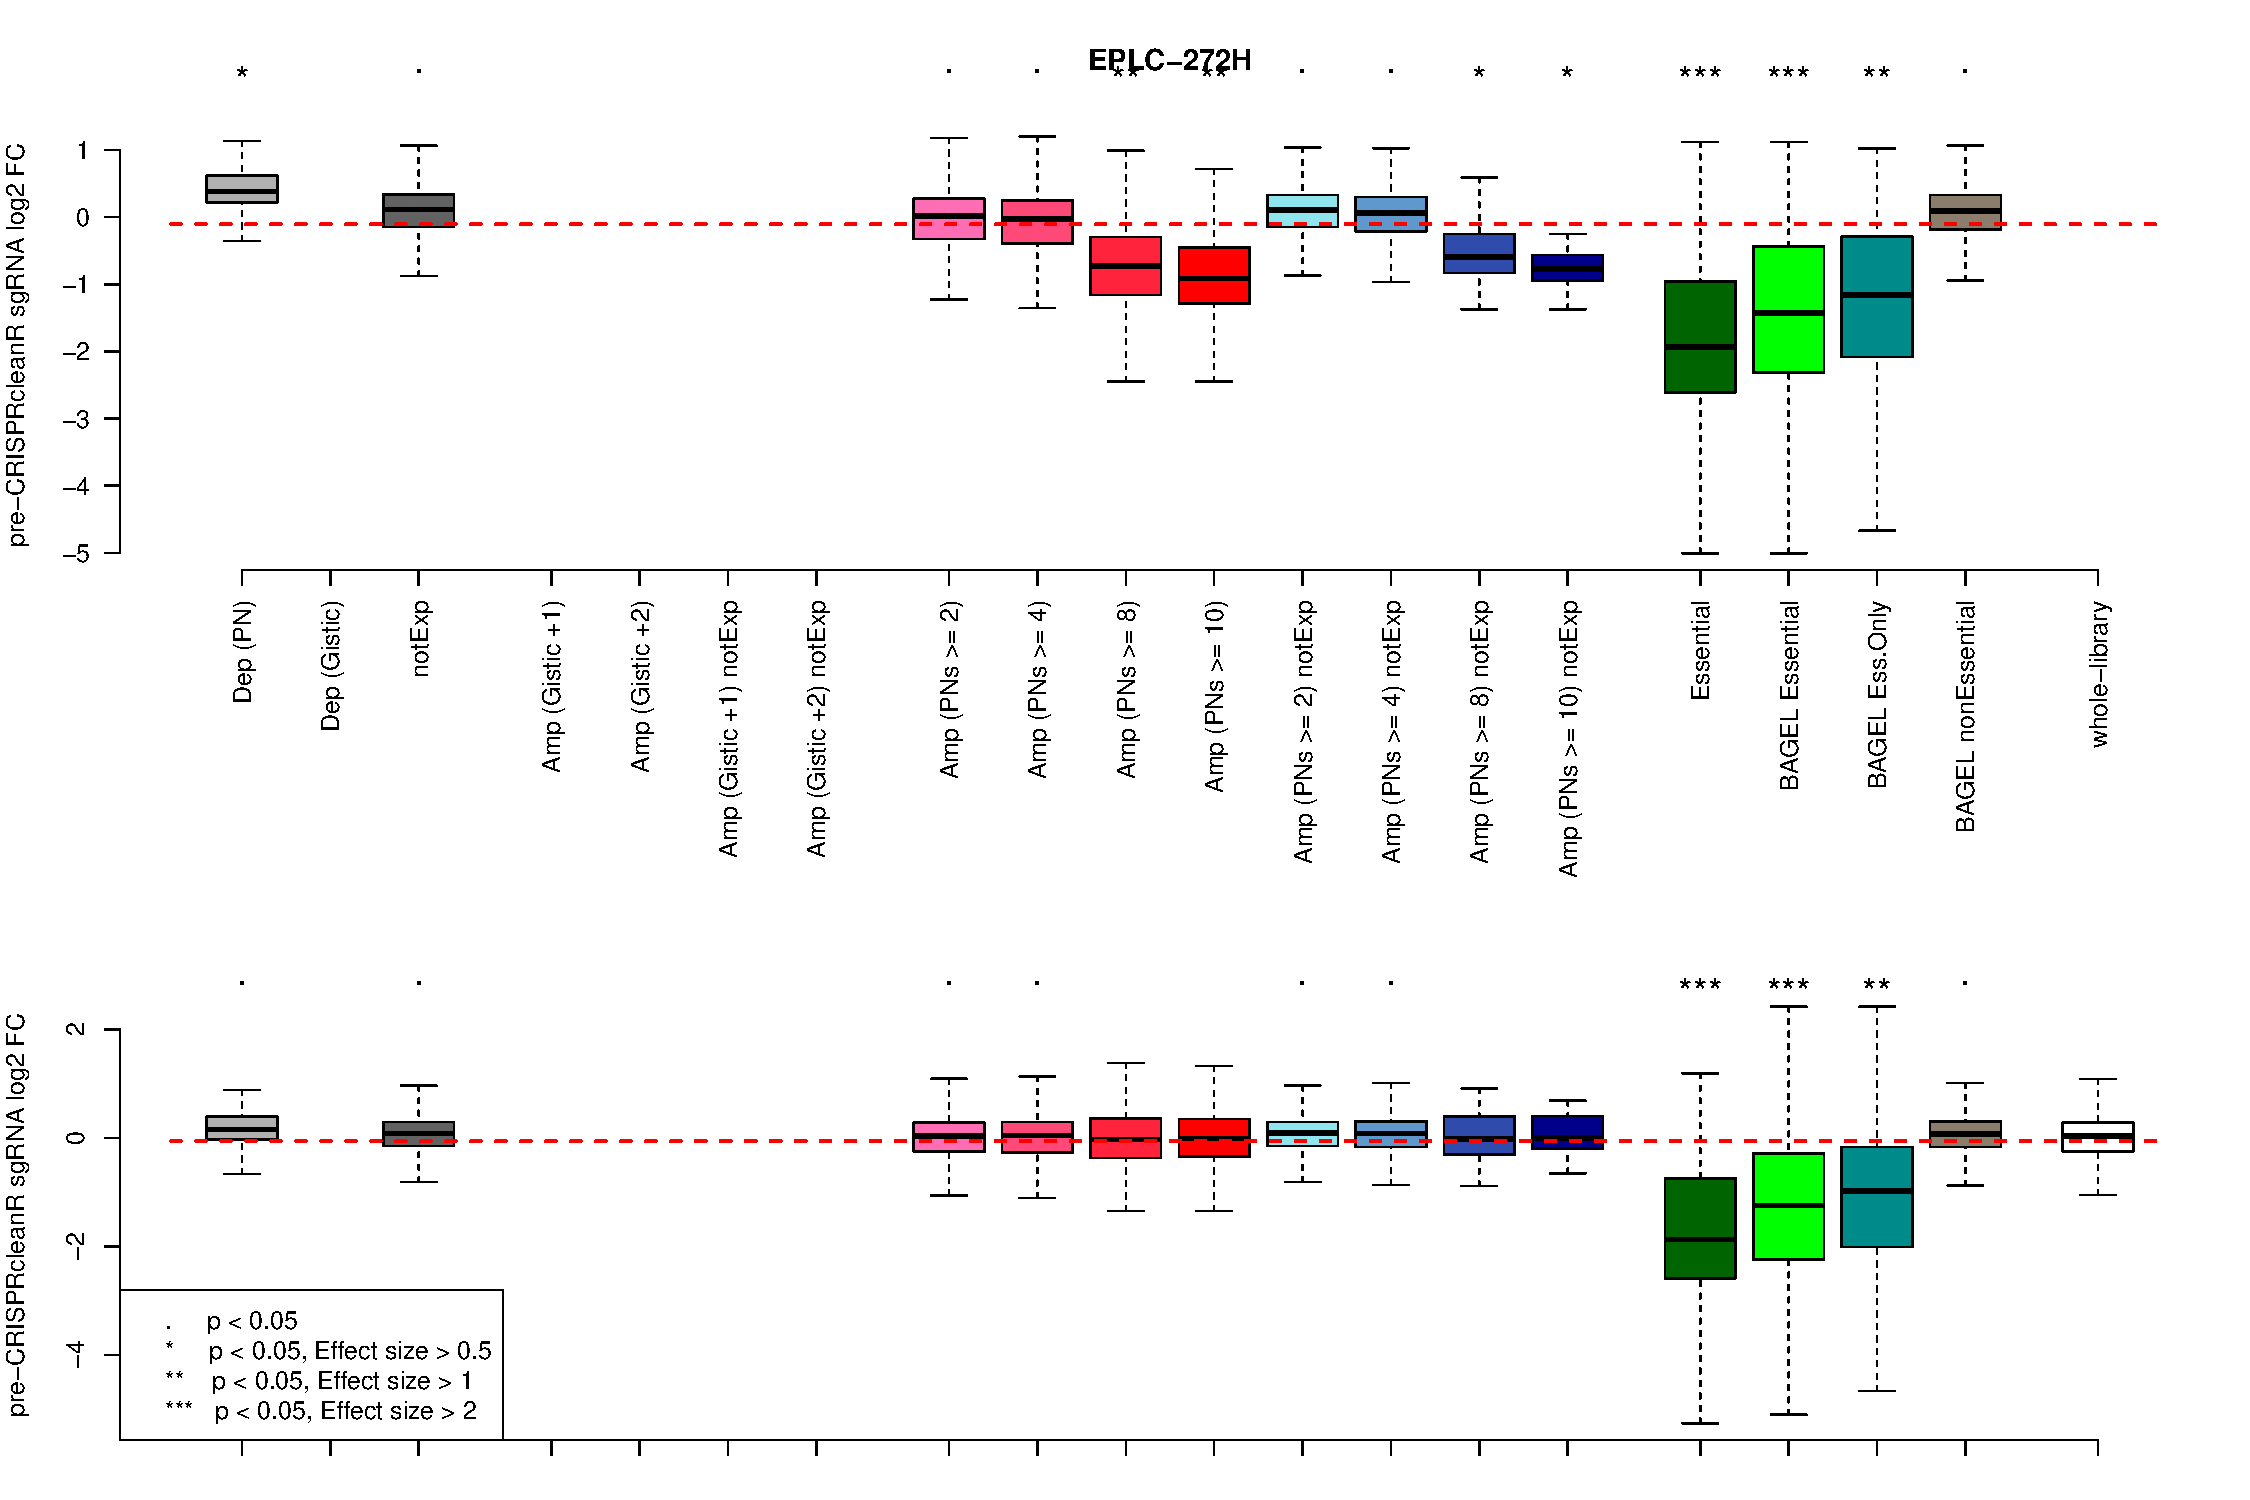
\includegraphics[width=130mm]{EPLC-272H_bp.pdf}
\end{figure}

\newpage
To inspect the variation induced by the CRISPRcleanR correction on the logFCs' distributions of sgRNAs targeting defined sets of genes prior/post\\ CRISPRcleanR correction, the following function can be also used (and will produce the following density plots):

\begin{knitrout}
\definecolor{shadecolor}{rgb}{0.969, 0.969, 0.969}\color{fgcolor}\begin{kframe}
\begin{alltt}
\hlkwd{ccr.perf_distributions}\hlstd{(}\hlstr{'HT-29'}\hlstd{,HT.29correctedFCs}\hlopt{$}\hlstd{corrected_logFCs,}
                       \hlkwc{libraryAnnotation} \hlstd{= KY_Library_v1.0)}
\end{alltt}
\end{kframe}
\includegraphics[width=\maxwidth]{figure/unnamed-chunk-33-1} 

\includegraphics[width=\maxwidth]{figure/unnamed-chunk-33-2} 

\includegraphics[width=\maxwidth]{figure/unnamed-chunk-33-3} 

\includegraphics[width=\maxwidth]{figure/unnamed-chunk-33-4} 

\end{knitrout}

\textbf{IMPORTANT:} The instructions provided regarding what CN/transcriptional data object to pass to the \texttt{ccr.perf\char`_statTests} apply also to this function.\\

Additional infos on how to use this function can be found in the user reference manual.

\subsection{Recall variations following CRISPRcleanR correction for reference, copy number amplified, and non expressed genes}

A final analysis that can be done with the CRISPRcleanR package in order to evalute the effect of its correction on the classfication recall for predefined gene sets can be performed by calling the function, which can work at the sgRNA 

\begin{knitrout}
\definecolor{shadecolor}{rgb}{0.969, 0.969, 0.969}\color{fgcolor}\begin{kframe}
\begin{alltt}
\hlkwd{ccr.RecallCurves}\hlstd{(}\hlstr{'EPLC-272H'}\hlstd{,EPLC.272HcorrectedFCs}\hlopt{$}\hlstd{corrected_logFCs,}
                  \hlkwc{libraryAnnotation}\hlstd{=KY_Library_v1.0)}
\end{alltt}
\begin{verbatim}
## [1] "No gistic CNA scores available for this cell line"
\end{verbatim}
\end{kframe}
\includegraphics[width=\maxwidth]{figure/unnamed-chunk-34-1} 
\begin{kframe}\begin{verbatim}
##                   BAGEL nonEssential BAGEL Essential Amp (PNs >= 8)
## pre-CRISPRcleanR           0.4405845       0.8282859      0.7921870
## post-CRISPRcleanR          0.4663982       0.8149893      0.5109027
##                   Amp (PNs >= 8) notExp
## pre-CRISPRcleanR              0.7447993
## post-CRISPRcleanR             0.4924973
\end{verbatim}
\end{kframe}
\end{knitrout}
 
as well as the gene level:

\begin{knitrout}
\definecolor{shadecolor}{rgb}{0.969, 0.969, 0.969}\color{fgcolor}\begin{kframe}
\begin{alltt}
\hlkwd{ccr.RecallCurves}\hlstd{(}\hlstr{'EPLC-272H'}\hlstd{,EPLC.272HcorrectedFCs}\hlopt{$}\hlstd{corrected_logFCs,}
                  \hlkwc{libraryAnnotation}\hlstd{=KY_Library_v1.0,}\hlkwc{GeneLev} \hlstd{=} \hlnum{TRUE}\hlstd{)}
\end{alltt}
\begin{verbatim}
## [1] "No gistic CNA scores available for this cell line"
\end{verbatim}
\end{kframe}
\includegraphics[width=\maxwidth]{figure/unnamed-chunk-35-1} 
\begin{kframe}\begin{verbatim}
##                   BAGEL nonEssential BAGEL Essential Amp (PNs >= 8)
## pre-CRISPRcleanR           0.4188711       0.8704539      0.8697322
## post-CRISPRcleanR          0.4570109       0.8627785      0.5156109
##                   Amp (PNs >= 8) notExp
## pre-CRISPRcleanR              0.8506553
## post-CRISPRcleanR             0.4828279
\end{verbatim}
\end{kframe}
\end{knitrout}

\textbf{IMPORTANT:} The instructions provided regarding what CN/transcriptional data object to pass to the \texttt{ccr.perf\char`_statTests} apply also to this function.\\

Additional infos on how to use this function can be found in the user reference manual.


\printbibliography

\end{document}
